\part{paper}

\section{A decision procedure for propositional projection
temporal logic with infinite models}
\textbf{无限模型下命题投影时间逻辑(PPTL)的决策过程}

\begin{enumerate}[(1)]
  \item 无限模型下命题投影时间逻辑(PPTL)的可满足性;
  \item PPTL 公式的决策过程;
  \begin{enumerate}
    \item PPTL 的范式;
    \item PPTL 的范式图;
    \item 根据公式转换为范式;
    \item 构造给定公式的范式图;
  \end{enumerate}
  \item 扩展 PPTL 的决策过程;
\end{enumerate}

\noindent
\fbox{
\textbf{Question}~~\textcircled{\footnotesize{1}}~~~\textbf{ITL, PTL, PPTL?}
}\\
\noindent ITL(Interval Temporal Logic) 区间时序逻辑, 规范和验证并发系统。

\noindent PTL 投影时序逻辑,相对于 ITL 扩展了 无限模型和投影操作。

\noindent PPTL 命题投影时序逻辑。


\noindent\textcolor{red}{决策过程是为了检查 PPTL 公式的可满足性条件。}


\subsection{PPTL}
\subsubsection{语法}
$P : :=~p~|~\bigcirc ~P~| ~\neg ~P~\left|~P_{1}~ \vee ~P_{2}~\right|~\left(P_{1},~ \ldots,~ P_{m}~\right) ~prj ~P$

$\bigcirc$, \textcolor{red}{$prj$}, 基本的时间运算符。


\noindent
\fbox{
\textbf{Question}~~\textcircled{\footnotesize{2}}~~~\textbf{PPTL 的 投影操作?}
}\\
\subsubsection{语义}

\begin{enumerate}
  \item state(状态):\\
    命题公式到真假集的映射。$B=\{t ~r ~u~ e, ~f~ a ~l~ s ~e\}, ~s ~: ~\operatorname{Prop}~ \longrightarrow~ B$
  \item interval(区间):\\
    有限无限区间的统一定义;\\
    区间长度比较操作:$=,<, \leq, \preceq$
  \item interpretation(解释):\\
    三元组:$\mathcal{I}=(\sigma, ~k, ~j)$ \\
    $\sigma$, 区间。\\
    $k \preceq j \leq|\sigma|$

\end{enumerate}


\subsubsection{运算法则}

\begin{figure}[!h]
  \centering
  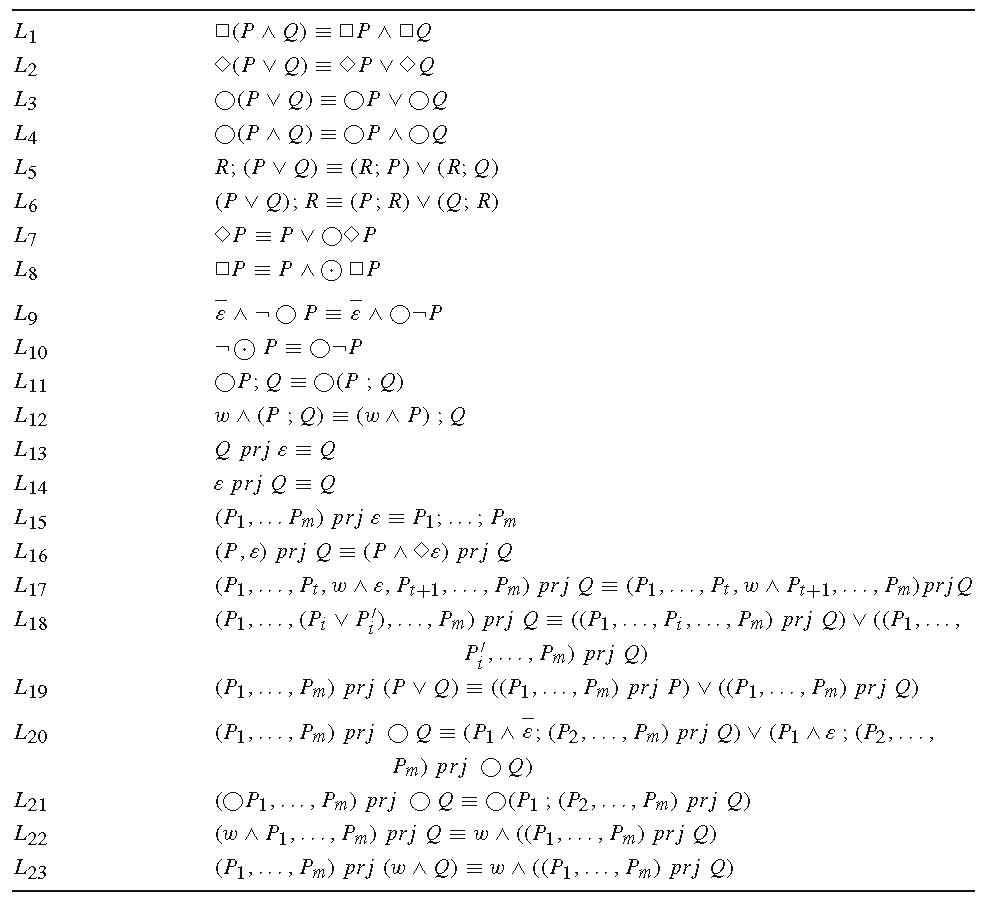
\includegraphics[width=1\textwidth]{law.png}
\end{figure}



